\newpage
\section{THEORETICAL PART}

%%%%%%%%%%%%%%%%%%%%%%%%%%%%%%%%%%%%%%%%%%%%%%%%%%%%%%%%%%%%%%%%%%%%%%%%%%%%%%%%%%%%%%%%
%%%%%%%%%%%%%%%%%%%%%%%%%%%%%%%%%%%%%%%%%%%%%%%%%%%%%%%%%%%%%%%%%%%%%%%%%%%%%%%%%%%%%%%%
In order to convert a real system consisting of individual molecules into a form that can be understood by a computer software, we must define individual parameters that are essential for describing mutual interactions of atoms. When describing real systems, it is usually necessary to consider a certain degree of approximation due to the possible computational complexity. In computational chemistry methods, we often encounter the so-called Born-Oppenheimer approximation, which is based on the decoupling of the motion of nuclei and electrons. The basis of the approximation is the orders-of-magnitude difference in mass between the electron and the nucleus. The latter thus move very slowly relative to the electrons and can thus be considered as a fixed point charge. This allows us to calculate the energy of a molecule as a function of the positions of the nuclei, in quantum chemistry we talk about the so-called Potential Energy Surface (PES), which is a function of 3$N$ coordinates, where $N$ is the number of nuclei. \cite{leach_molecular_2001} 

For small systems it is possible to calculate the PES based on quantum chemistry methods using reasonable resources, for very large systems this is not yet realistic. We therefore introduce a classical-mechanics set of analytic functions, yet empiric parameters called the Force Field (FF), which enable to evaluate the energy of simulated systems depending on the positions of the nuclei. Methods based on the use of such Force Fields are called molecular mechanics, which are applied especially when quantum phenomena are not of great importance and we can use classical mechanics approach or big amorphous systems where quantum-based calculations would be extremely expensive and resource taking. \cite{monticelli_force_2013}

\subsection{Force fields}
The total energy calculated using the force field can be broken down into two contributions, a binding and a non-binding term, which are further expanded in Equations \ref{eq:ff2} and \ref{eq:ff3}.

\begin{comment}
	\begin{equation}\label{eq:ff1}
		E_{\text{total}} = E_{\text{bonded}} + E_{\text{nonbonded}}
	\end{equation}.
\end{comment}


\begin{equation}\label{eq:ff2}
	E_{\text{bonded}} = E_{\text{bond}} + E_{\text{angle}} + E_{\text{torsion}}
\end{equation}

\begin{equation}\label{eq:ff3}
	E_{\text{nonbonded}} = E_{\text{electrostatic}} + E_{\text{Van der Walls}}
\end{equation}

%To get a better idea of what lies behind the individual terms, visualization of the corresponding mechanistic degrees of freedom is in the Figure \ref{fig:ff}. OBRÁZEK VYTVOŘÍM VLASTNÍ V PODOBNÉM DUCHU----
%
%\begin{figure}[htb!]
%	\centering
%	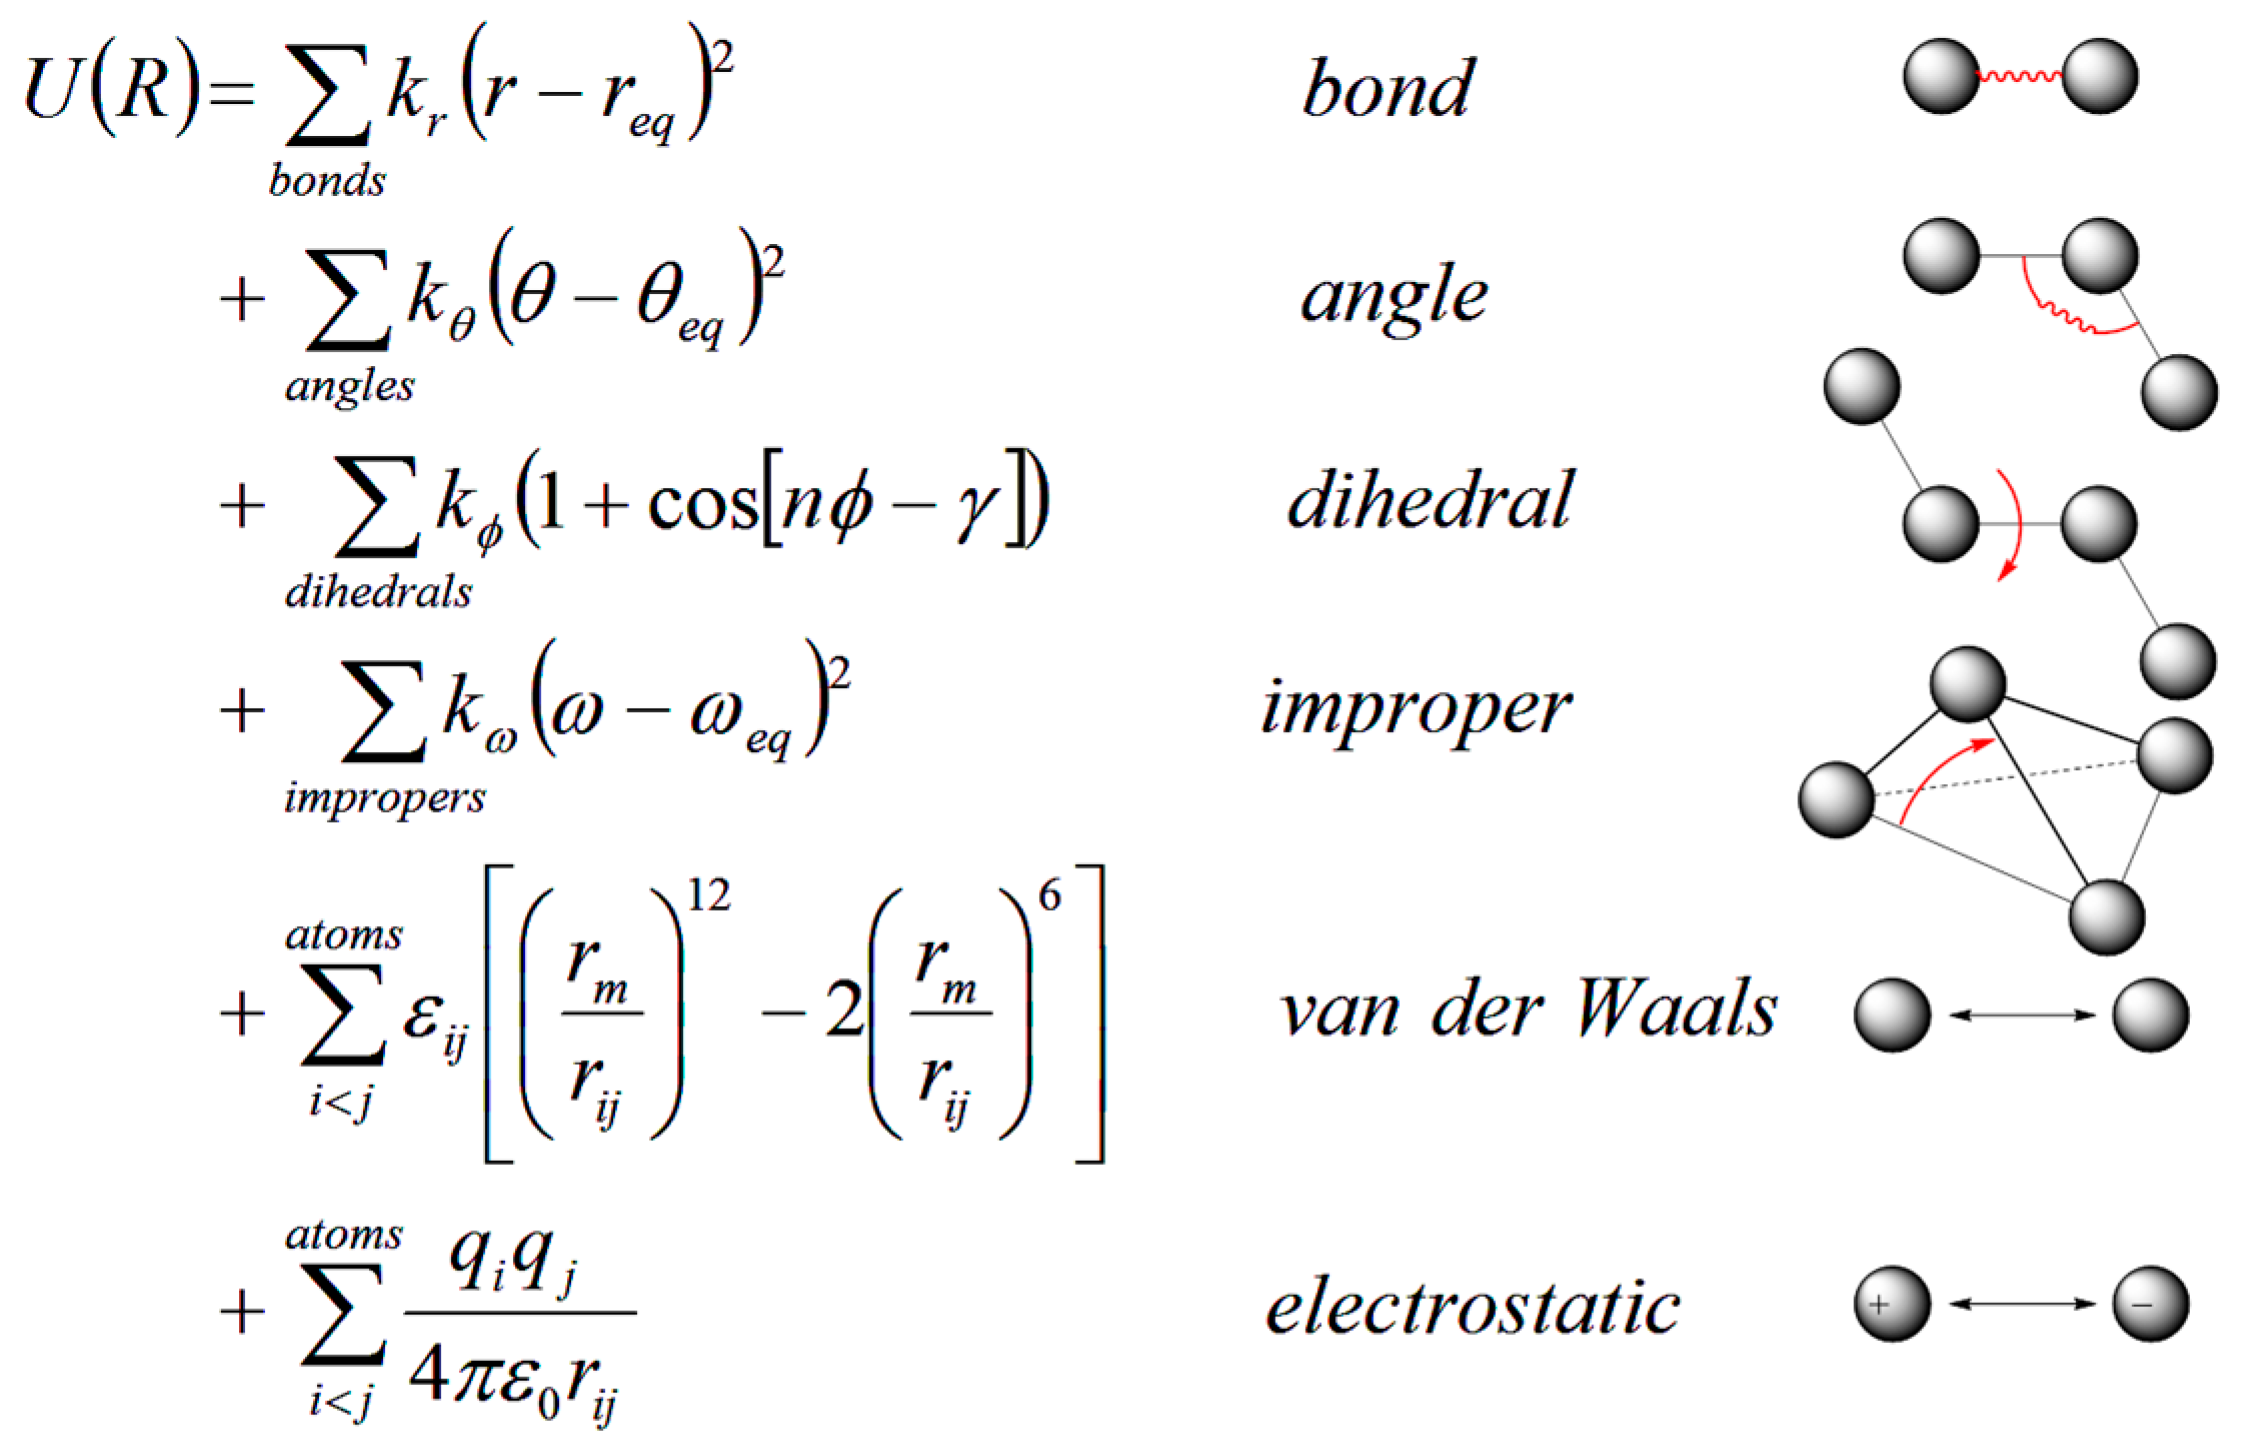
\includegraphics[width=1.0\linewidth]{img/ff.png} 
%	\caption{caption}
%	\label{fig:ff}    
%\end{figure}  

By the level of functional description (number of terms) of the interactions in the force field, we distinguish force fields of three classes. Class 1 force fields contain the 5 terms mentioned in the two equations above (bond, angle, torsion, Lennard-Jones and electrostatic), examples of such FF are the DREIDING, AMBER \cite{brooks_charmm_2009}, GAFF and OPLS. In addition, class 2 force fields include bond-bond and bond-angle coupling terms, anharmonic terms simultaneously with all class 1 terms, examples of such fields are PCFF or ReaxFF.  The third class includes fluctuations of charge distribution in time (charge polarization effect), and they are called polarizable FF. \cite{vanommeslaeghe_molecular_2014}

During the parameterization of force fields (FF), we start from the assumption of transferability,  similar chemical groups of different molecules interact in the same way. When constructing a force field for large molecules, we can use parameters obtained from data for small molecules, which are much more easily graspable and contain the same functional groups. \cite{monticelli_force_2013} In model development, our aim is to achieve the most universal description of the system while still closely corresponding to its actual state. This can be facilitated by employing higher-order terms; however, incorporating anharmonic and cross terms introduces the need for a greater amount of FF parameters. We strive to avoid situations where we employ an overly adapted and detailed model that merely reproduces inserted information without providing any predictive capabilities. \cite{vanommeslaeghe_molecular_2014}

According to the level of parameterization, there are 3 basic types of force fields. In the first case, where the parameters are determined for each individual atom in the system, including hydrogens, we speak of an all-atom force field. A united atom force field is one where we parameterize the individual functional groups (interaction centers), such an interaction center could be for example a methyl group. The third type of force field is coarse grained, used mainly for protein and polymer simulations, offering higher computational efficiency for long simulations of large molecules by grouping them into "superatoms". \cite{da_silva_are_2020}

\subsubsection{OPLS force field}

Optimized Potential for Liquid Simulations (OPLS) force field was developed by William L. Jorgensen \cite{jorgensen_opls_1988} at Purdue University and later at Yale University based on previously released Assisted Model Building and Energy Refinement (AMBER) force field developed by Peter Kollman's group. \cite{cornell_second_1995} The OPLS force field consists of following terms written in Equation \ref{eq:opls}. 
	
	\begin{equation}
		\begin{aligned}
			U_{\text{OPLS}} = & \sum_{\text{bonds}} \frac{1}{2} k_b(r-r_0)^2 + \sum_{\text{angles}} k_{\theta} (\theta-\theta_0)^2 \\
			& + \sum_{\text{dihedrals}} \Biggl( \frac {V_1} {2} \left [ 1 + \cos (\phi) \right ] + \frac {V_2} {2} \left [ 1 - \cos (2\phi) \right ] 
			+ \frac {V_3} {2} \left [ 1 + \cos (3\phi) \right ] + \frac {V_4} {2} \left [ 1 - \cos (4\phi) \right ] \Biggr) \\
			& + \sum_{i<j}^N 4\epsilon_{ij} \left[ \left( \frac{\sigma_{ij}}{r_{ij}} \right)^{12} - \left( \frac{\sigma_{ij}}{r_{ij}} \right)^6 \right] + \sum_{i<j}^N k_{ij} \left( \frac{1}{r_{ij}^m} - \frac{1}{r_{ij}^n} \right)
		\end{aligned}
		\label{eq:opls}
	\end{equation}
	
	where,
	\begin{itemize}
		\item $U_{\text{OPLS}}$ is the total OPLS potential energy,
		\item $i$ and $j$ denote different atom types,
		\item $N$ is the total number of atom pairs,
		\item $\epsilon_{ij}$ is the depth of the potential well,
		\item $\sigma_{ij}$ is the finite distance at which the inter-particle potential is zero,
		\item $r_{ij}$ is the distance between atoms $i$ and $j$,
		\item $k_{ij}$, $m$, and $n$ are additional parameters.
	\end{itemize}
	
\textbf{Bonds and angles} are described as harmonic oscillators in OPLS FF. The equilibrium parameters are obtained by structural methods, such as x-ray diffraction NMR experiments. The values for force constants are then fitted to experimental data taken from vibrational spectroscopy. In Figure \ref{fig:bond} is the visualization of the constants.

\begin{figure}[htb!]
	\centering
	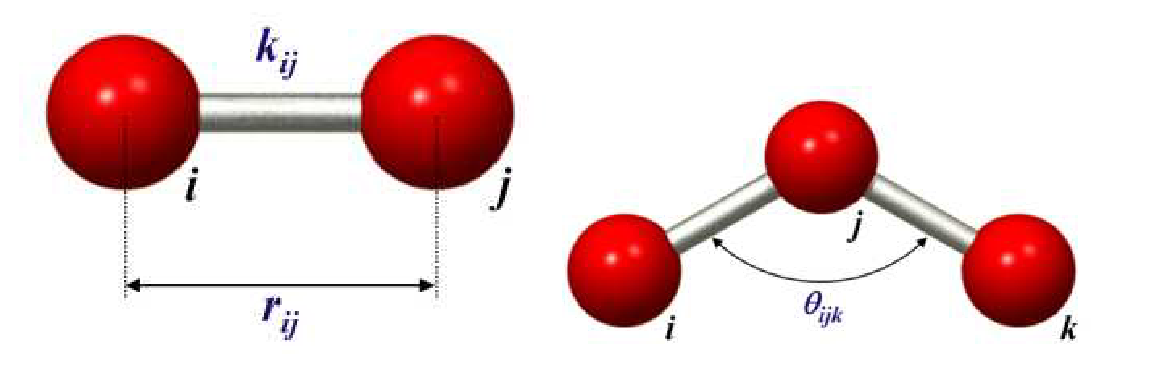
\includegraphics[width=1.0\linewidth]{img/bond_angles.png} 
	\caption{caption}
	\label{fig:bond}    
\end{figure}   

\textbf{Dihedral angles} could be calculated by two different approaches. First option is to obtain the dihedrals in large molecules from optimization the potential in small molecules containing the same dihedral. calculate and optimize the dihedral potential for simplest possible molecule. Dihedrals are obtained by ab initio calculations procedure. 

\textbf{Charges} parametrization is also done by ab initio methods. When we are using the classical FF, the charges used to calculate the Coulomb potential remains the same during the simulations. Due to that, it is crucial to obtain the charges from equilibrium state of the molecules in order to avoid any errors from having the charges taken from structures with higher energy. When obtaining the charges, the first step is to optimize the geometry using the appropriate level of theory, meaning the basis set to be better or equal to 6-31G. Commonly used method to achieve the charges is CHELPG (CHarges from ELectrostatic Potentials using a Grid based method), based on adjusting the partial charges at the centers of the nuclei in order to get the best representation of the electrostatic potential given by the wave functions. Calculation of the charges are often done using higher-level methods and basis sets such as B3LYP/cc-pVTZ or HF/6-31G**.

\textbf{Van der Waals} forces are most often represented by the Lennard-Jones (LJ) potential. The functional form with the illustration is in Figure \ref{fig:lj}. Lennard-Jones potential is a combination of two terms, repulsive term describes the Pauli repulsion at short distances and the attractive term describes the London dispersion force. The $\epsilon$ values are adjusted to experimental values of heats of vaporization and $\sigma$ parameters are adjusted to experimental densities and structural data.

\begin{figure}[htb!]
	\centering
	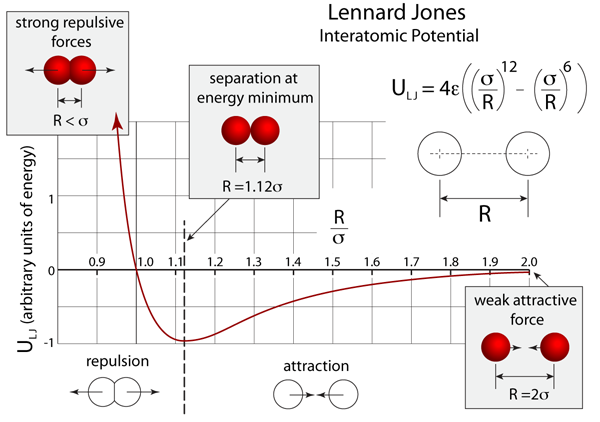
\includegraphics[width=1.0\linewidth]{img/lj.png} 
	\caption{caption}
	\label{fig:lj}    
\end{figure} 

\subsubsection{Charges and dipoles}

\subsubsection{Polarizability}



\subsection{Periodic boundary conditions}
Due to the computational complexity, we are focused on only small region of a very complex real system.  In order not to introduce errors caused by the boundaries of the system and interaction on them, we introduce periodic boundary conditions (PBC). This method is based on surrounding the simulated system with periodic images, thus achieving an approximation by a surface less system. We choose a shape of the simulation box that can be used to fill the space without problems, in our case a cubic box. For simulations in three dimensions, we usually introduce PBCs in the direction of all axes, which means that our simulated box is surrounded on all sides by a total of 26 replicas of the system. The behavior of the system is the same in all replicas, so we must include all the particles appearing in the replicas when calculating the pair interactions. The calculations of such interactions are very demanding, but due to their nature they do not need to be calculated over large distances, so we introduce a reasonable cut-off distance beyond which we no longer consider those pair interactions.

From the preceding paragraphs it is evident that the main problem of time complexity of simulations is the evaluation of non-bonding energies. While the contributions for the coupling parameters increase linearly with the system size, the non-coupling terms show a quadratic increase with the system size. A common tactic to reduce computational time is to set cutoff distances beyond which we no longer consider these contributions. By neglecting the contributions at long distances, we introduce small numerical deviations for each pair, but the cumulative effect when all pairwise interactions are summed introduces larger deviations into the simulations. We chose 12 A as the optimal cutoff in our simulations, however, theory suggests that WDW interactions are negligible beyond about 20 A. 

Translated with DeepL.com (free version)
\subsubsection{Ewald}
\subsubsection{PPPM}
\subsubsection{Cutoff}
\subsection{Conditions}


\subsection{Molecular dynamics}
The molecular dynamics method is based on solving the equations of motion of classical Newtonian mechanics for atoms. Let us choose the assumption that the interaction potential $U$ is continuous and differentiable. The force acting on the $i$ particle can thus be written as an equation \ref{sila1} 
\begin{equation}\label{sila1}
	f_i=-\frac{\partial U(r^N)}{\partial r_i}, \qquad i=1,...,N.
\end{equation}

In molecular dynamics, we are focused on the time development of the model. In other words, we are looking for the trajectory of the solution of the respective systems of differential equations. In Newtonian mechanics, acceleration is directly related to forces through the equations of motion. Formally, we can write the equation \ref{sila2}
\begin{equation}\label{sila2}
	\Ddot{r_i}=\frac{f_i}{m_i}, \qquad i=1,...,N,
\end{equation}
where the second time derivative of the positions appears on the left side. The equation \ref{sila2} is a system of 3$N$ ordinary differential equations for a set of $N$ atoms. As initial conditions, we usually choose the knowledge of all atomic positions $r_i$ and velocities $\dot{r_i}$ at the initial time $t=t_0$. 

We solve equation \ref{sila2} using the finite difference method when we track the desired solution in the form of the function $r_i(t), i=1,..,N$, in the time interval $[t_0,t_{max}]$ at discrete points of the form $t=t_0+kh$, where $h$ is the integration step and $k$ is a non-negative integer.

To find a solution, it is necessary to calculate the forces acting on individual particles at each step of the simulation. One of the methods that is applied in this area is the Verlet integration method. It is a simple and very effective method that provides sufficiently accurate results in the physico-chemical context. Its great advantage is the time-reversibility and the conservation of the total energy of the system~\cite{mdskripta}.

\subsubsection{Verlet integration}
Verlet integration method is a numerical method for integrating the equation \ref{sila1}. We express the second derivative using finite differences. From the second-order Taylor expansion $r_i(t\pm h)$ centred at $t$, we obtain the formula
\begin{equation}\label{sila3}
	\Ddot{r_i}=\frac{r_i(t-h)-2r_i(t)+r_i(t+h)}{h^2},
\end{equation}
binding values at three points in a row ($t-h$, $t$ and $t+h$). We will use this characteristic to calculate $r_i(t+h)$. By substituting \ref{sila3} into \ref{sila1} we get 
\begin{equation}\label{sila4}
	r_i(t+h)=2r_i(t)-r_i(t-h)+h^2\frac{f_i(t)}{m_i}.
\end{equation}
In this formulation, we are able to calculate the new positions at time $t+h$ from knowledge of the forces at time $t$, the positions of the particles at time $t$ and the previous time $t-h$. The time reversibility of the method is clearly visible here. The advantage is that the force is calculated only once in each step of the simulation. For the position preceding the initial position ($r_i(t_0-h)$), we can use the expansion \ref{sila5}
\begin{equation}\label{sila5}
	r_i(t_0-h)=r_i(t)-h\dot{r_i}(t_0)+h^2\frac{f_i(t_0)}{2m_i}.
\end{equation}

\subsubsection{Constraint dynamics}

When integrating equations of motion, we often impose constraints on certain aspects of molecular geometries. The main reason is to enable using a longer simulation time step. If we simulate with a too large time step, we introduce large errors into the simulations, leading in extreme cases to a crash of the simulation. The calculated particle positions at time $t+h$ may lead to overlapping of particles, the calculated force acting on the particles may divert from physically reasonable configurations. Conversely, the use of inappropriately short simulation steps reduces the efficiency of the simulations (the most computationally and therefore time consuming element of the simulations is the calculation of the forces when integrating the equations of motion). \cite{mdskripta} The criterion determining the optimal step length is the accuracy of the conservation of total energy. The step length can be determined by an Nyquist-Shannon \cite{shannon_communication_1949} sampling theorem that says that the time step must be half or less of the period of the quickest dynamics exhibited in the system. Thus, for systems containing very light hydrogen atoms, we can either artificially increase the mass of the hydrogen atom while redistributing the masses of the other molecules to conserve the overall mass of the molecule, or fix the bond angles or bond lengths terminating in the hydrogen atoms. It is the fixation of hydrogen bond lengths that is most often implemented in the Verlet method, using an algorithm called SHAKE. 

The SHAKE algorithm is based on Verlet's integration method and is iterative. The first step is to initialize the initial velocities and positions of the atoms, then calculate the positions using Verlet's method without considering bond length constraint. We then create the $\lambda$ correction of the atom positions to constrain the bond length. Fixing the bond length allows us to use a longer time step (we are no longer limited by the motion of very light particles) and, unlike fixing angles, does not introduce large deviations in the simulations.

\subsection{Measuring the properties}
\subsubsection{MSD}
\subsubsection{RDF}
\subsubsection{Glass transition temperature}